This chapter motivates and defines \emph{Persistent Memory Consistency}.
This should be considered future work and I welcome feedback.
I first define the problem and then give examples of persistent memory consistency models.
In the next chapter I give examples of programming patterns, why they require relaxed persistent consistency models, and possible optimizations.

\section{Introduction}
\label{sec:PMC:Intro}

Future NVRAMs will provide a persistent store with the programming interface of modern main memories.
While such technologies could revolutionize the design of recoverable systems and durable storage, questions remain regarding device performance and the NVRAM programming model.
Chapters~\fixme{ref} and~\fixme{ref} consider an abstract \emph{persist barrier} capable of enforcing persist order or blocking until previous persists complete.
Instead of considering an implementation or exact semantics of these barriers, I instead looked at the effect average persist barrier latency had on OLTP software design.
This project delves into the details of persist barriers, considering their implementation, performance impact, and programming model.

Persist barriers exist as a tool for programmers to ensure correct persistence behavior, while at the same time improving performance.
Imagine an NVRAM model where persist barriers do not exist.
Without persist barriers, all persists must truly occur in program order for the programmer to reason about persistent state.
This is in fact a popular model for DRAM programming, but the volatile semantics of DRAM writes to execute to fast caches.
NVRAM persists, on the other hand, must always execute to a long latency memory; executing all NVRAM persists in-order will introduce frequent, substantial stalls.
Persist barriers remove these stalls by allowing all persists between barriers to occur in parallel.
This is a prime example of using a more sophisticated programming model to provide performance optimizations.

An additional mechanism to reason about persistent state is to flush select cache lines or flush the entire cache, either blocking until all data persists or receiving an acknowledgement/interrupt.
This model most closely matches the existing disk interface -- The programmer invokes system calls to write individual pages and then calls a sync system call on files.
However, this is a poor match for memory, where the programmer often has little control over how data is laid out in cache lines (nor should the programmer have to reason about cache architecture).
Instead, we would like a more natural approach to reasoning about persistence that fits existing memory-programming models.

Additional questions remain when persistent memory is shared between threads or processes.
Currently, memory consistency models define how threads communicate and what barriers are necessary to ensure proper behavior.
Memory consistency models exist because processors prefer to run instructions out of order -- a pervasive optimization that significantly complicates multi-threaded programming.
While consistency models control the order in which threads observe reads and writes, there is no similar definition for the order in which persists occur, or how persist order is enforced across communicating threads.
Furthermore, persistent memories often care about the actual timing of persists, not just relative ordering -- for example, system calls must make sure that all previous persists have completed before notifying the user.
In this case there is no alternative but to block until all data persists.
These mechanisms are not present in existing consistency models.

While memory consistency models provide a starting point for considering persistent consistency models, the performance differences of volatile memory systems/DRAM and NVRAM will require new programming models for NVRAM.
In fact, the consistency and persistence models may be de-coupled.
That is, the rules that define load and store order might be different between how \emph{values} are communicated and how \emph{persist order} is enforced.

I wish to extend memory consistency models with persistence semantics to address these concerns.
The goals are to determine how multi-threaded consistency interacts with persistence, how to relax consistency/persistency models to provide high performance and an easily programmable interface, and identify programming patterns likely to cause NVRAM bottlenecks alongside potential optimizations.
All of these will eventually lead to the design of new persistent memory consistency models and implementations, yet that is most likely outside the scope of this project.

The remainder of this chapter provides a brief background of memory consistency models before considering simple examples of persistent memory consistency models.
In addition, I examine previous work, highlighting strengths and weaknesses, and placing it into my persistent memory consistency taxonomy.

\section{Memory consistency models}
\label{sec:PMC:MemoryConsistency}

This section provides a background on memory consistency models, focusing on two simple models: Sequential Consistency (SC) and Total Store Order (TSO).
For the remainder of this section I am referring solely to volatile writes without considering for NVRAM persists.
This discussion assumes that caches are completely coherent -- that is, any two accesses to a cache line (by any core/thread), where at least one access is a store, have a total order.
While incredibly relaxed memory models may allow stale cached values to be read, I do not consider that here.

Consistency models define the order that threads observe loads and stores.
While every thread observes its own execution in program order, it may appear that remote threads execute out of order.
Processors (and compilers) are free to reorder instructions to accelerate performance so long as they produce equivalent results.
When examining a program ordering restrictions can be observed through register and memory dependencies.
However, it is much more difficult to observe memory dependencies between threads.
Loads and stores that are independent from a single-threaded point of view may in fact interact with other threads.
Reordering these memory accesses can result in unintended program behavior.

Two popular solutions to this problem are to 1) force all threads to observe the loads and stores of other threads in a globally defined order (SC) or 2) relax this guarantee, introducing memory barriers that allow the programmer to enforce a certain order when necessary (e.g., TSO).
While relaxing consistency may provide higher performance, it places a greater burden on the programmer to correctly use memory barriers.

\textbf{Sequential Consistency.}
Sequential consistency provides the most intuitive programming model, yet necessarily the worst performance (although modern techniques involving speculation provide high performance).
All loads and stores across threads appear in some globally consistent order that is an interleaving of the program order of all threads.
There is no need for the programmer to consider that memory instructions might reorder or use memory barriers.

\textbf{Total Store Order.}
TSO provides greater performance than SC at the cost of requiring the programmer to insert memory barriers.
Most memory operations are still observed to occur in program order: 1) stores may not reorder with other stores, 2) loads may not reorder with other loads, and 3) a store that occurs after a load may not reorder and appear to occur before that load.
This guarantees that all stores occur in a globally consistent sequentially order.
However, loads that occur after a store in program order may reorder and bypass the store, appearing to occur before the store.
The justification for doing this is that stores are typically not on the application's critical path -- they simply write into the cache and do not insert delays.
Loads, on the other hand, may cause delays if they miss in the cache and must execute to a higher level cache or main memory.
These loads must start as soon as possible to minimize delays.

The programmer is responsible for locating any code where allowing a load to bypass a store causes an incorrect result.
In this case, a barrier is provided by the architecture to force all loads to delay until the store appears to other threads (or rerun those loads if some other thread stores to those addresses).
I believe a similar trade off exists for persistence -- in order to gain performance we relax persistence constraints so that persist order may not match program order and may not appear as a valid interleaving of all persists.

\section{Persistent Memory Consistency Models}
\label{sec:PMC:PersistenceModels}

While memory consistency models control the order that loads and stores are observed across threads, they give no guarantees on persistence.
I outline several persistent consistency models, starting with a constrained, strong model, and then considering more relaxed models.
The purpose of these models is to provide correctness by defining the allowable persistent states during execution.
Any implementation may only allow these states.
Implementations are free to insert further restrictions, disallowing other persistent states.
However, specific implementations are outside the scope of this proposal.
I welcome any feedback.

\subsection{Persistent Sequential Consistency}
\label{sec:PMC:PersistenceModels:PSC}

The first model couples persistence to the sequential consistency model as Persistent Sequential Consistency (PSC).
All loads and stores (including persists) appear to occur in a globally defined order as an interleaving of valid program orders.
Whereas volatile memory systems control this solely by controlling the order in which memory actions become visible from each processor, NVRAM used for recovery must treat every point in time as a possible failure, observing the persistent state.
Achieving a globally consistent persist order requires that persists \emph{actually} occur in-order from each thread, or that sequential batches of persists occur atomically, so that no failure may observe an intermediate state (NVRAM's atomically persistable size is likely to be small -- 8 bytes usually assumed).
Additionally, all data sharing propagates ordering dependencies between persists.

Consider Figure~\fixme{ref}.
The letters correspond to persistent variables, and all are initialized to 0.
Assuming threads execute under a sequential consistency model (i.e., they observe shared values from that model) and persist orders are enforced according to the PSC model, at no point may we observe that A=1, C=1, and B=0.
Doing so would violate the model by allowing thread 1 to observe a persist from thread 2 (B=1) and then persist an additional value before B persists.
Even if the program executes according to SC, persistence order must also be observed.

The problem with PSC is that all persists are ordered.
If persist latency is large (expected to be at least hundreds of nanoseconds up to several microseconds) every persist will incur this penalty; there is no opportunity to execute persists from the same thread in parallel.
While persists across threads may occur in parallel, sharing introduces additional dependencies, increasing delays further.
The next model relaxes the multi-threaded constraint.

\subsection{Local Persist Order}
\label{sec:PMC:PersistenceModels:LPO}

This model considers that thread communication and data persistence should not always occur at the same granularity.
Imagine, as an example, the \GroupCommit design of Chapters~\fixme{ref} and~\fixme{ref}.
In that design we required a volatile staging buffer, separate from the primary NVRAM store, where batch updates occured.
Only at the end of the batch would we copy the original batch data to an undo log and persist batch updates in-place to NVRAM.
An alternative design that omits this staging buffer would allow updates during a batch directly to the NVRAM address space.
However, every operation must first check if the address region being modified is protected by a segment of the undo log, and if it is not create and persist the necessary undo first.
Once a region of memory is protected by undo, threads may update the NVRAM store in-place, and the memory system is free to persist any values (or not) -- until the end of the batch there are no semantic constraints on the value in NVRAM.
Of course, when the batch ends the NVRAM store must necessary arrive at the final persistent version of the batch before transactions commit.

Consider this design under PSC -- all persists within a thread occur in-order, and whenever data is shared a persist order is enforced.
However, there is no need to enforce a persist order across threads.
Data may persist in any order so long as 1) associated undo log persists first and 2) the batch manager receives proper acknowledgement at the end of the batch that all data has successfully persisted.
Additional cross-thread dependences introduce unnecessary persist-order constraints that increase the critical path of persists, limiting persist throughput.

I relax cross-thread dependences in a model called \emph{Local Persist Order} (LPO).
All persists within a thread continue to execute in-order, as in sequential consistency.
The persistent state at any point in time represents correct execution according to the underlying consistency model (which can be SC, TSO, etc.).
However, each thread may have progressed persistent state to various degrees in ways that may violate PSC.
For example, again considering Figure~\fixme{ref}.
It is now possible to observe A=1, C=1, but B=0.
This would occur if \emph{consistency execution} observed thread 2 executing entirely before thread 1, but thread 1 persisting entirely before thread 2 (which is allowed according to the LPO).

The previous situation may be avoided by using explicit persist barriers.
There are many types of barriers, with varying implementations.
I will simply highlight a few here.
A thread may enforce that all local persists occur before any other thread observes them and then persists itself in a \emph{persist send}, useful for communicating persistence to another thread.
A thread may enforce that all remote persists occur before subsequent local persists in a \emph{persist receive}, useful for reading persists from remote threads.
Both of these may be combined in a \emph{persist total fence}, allowing a thread to completely order all persistent actions with other threads.
While these define persistent state, we still rely on an underlying consistency model to determine what \emph{values} are communicated.
My batching example may use these by having all threads participating in the batch access some pre-determined memory address and emitting a persist send at the end of the batch.
Once the batch manager is certain all threads have accessed this memory it accesses the pre-determined memory address itself and inserts a persist receive, ordering the persists from all other threads before any subsequent persists from the batch manager.
The batch manager is then free to invalidate the log, committing the batch.
The use of persist barriers ensures that all store data persists before the batch commits, but during batch execution false cross-thread persist dependences do not limit execution.

\begin{figure}
\centering
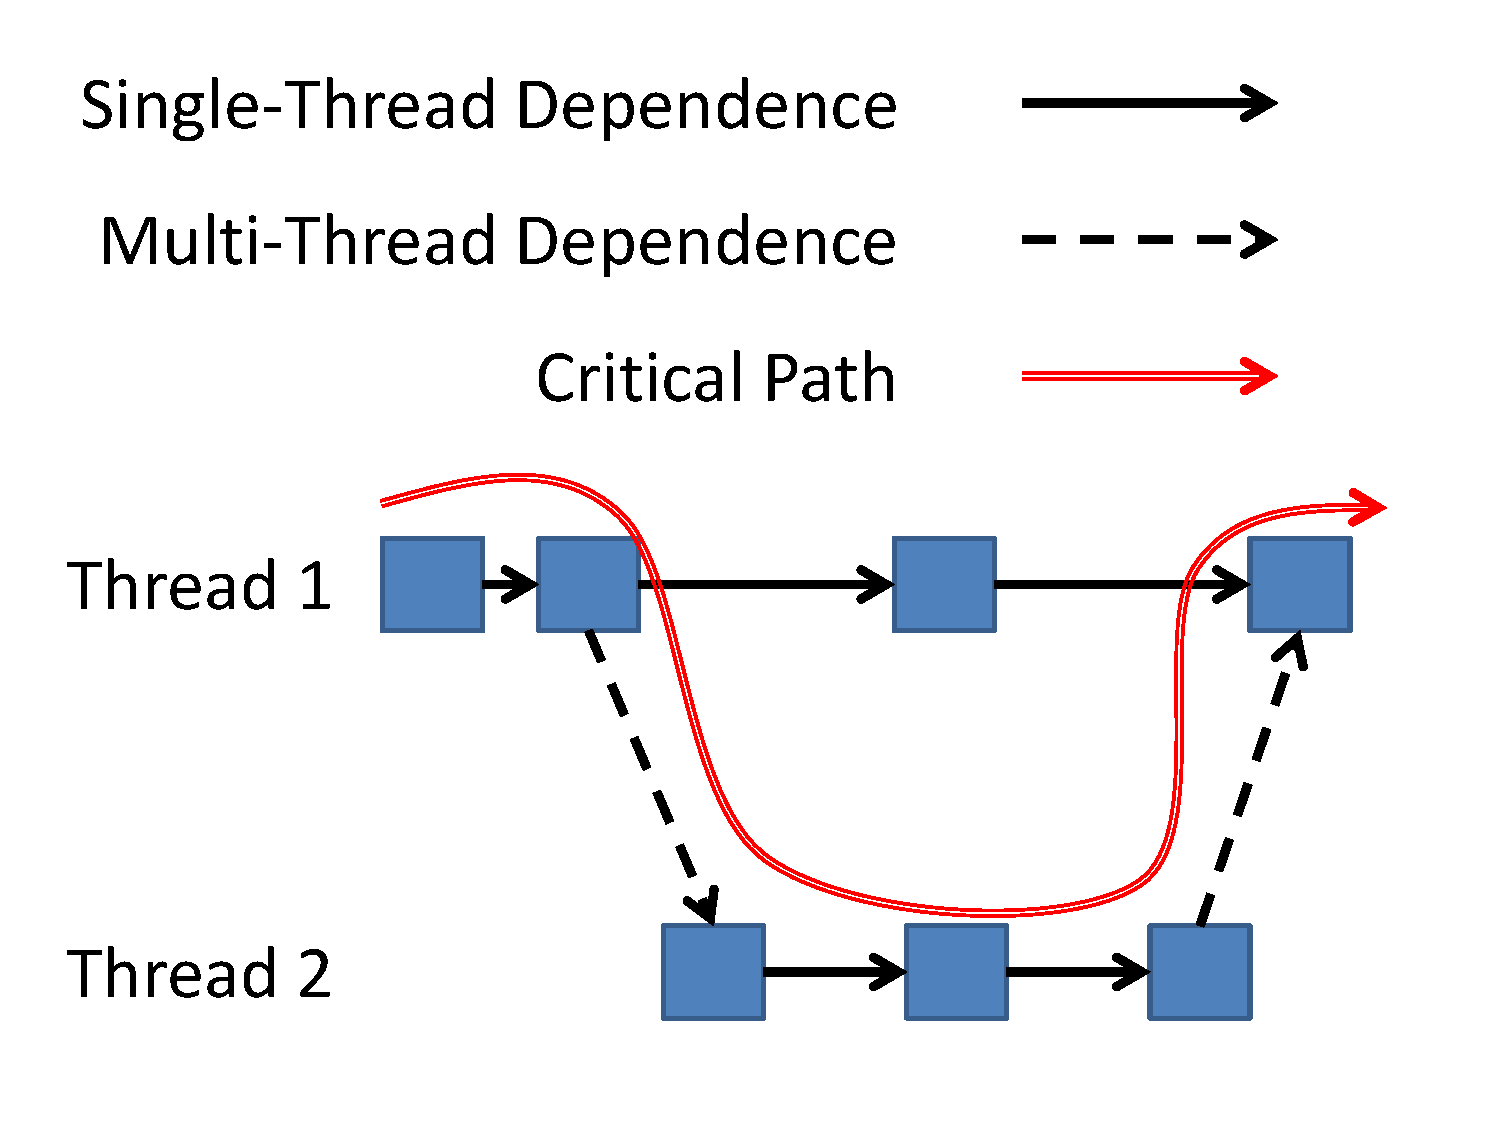
\includegraphics[width=.7\textwidth]{PMC/LPO.pdf}
\caption{\textbf{Local Persist Order.} LPO removes cross-thread persist dependencies, reducing persist critical path (PSC critical path traced in red).  Enforcing cross-thread dependencies requires explicit persist barriers.}
\label{figure:LPO}
\end{figure}

LPO potentially improves performance by minimizing the critical path of persist dependencies, shown in Figure~\fixme{ref}
Data sharing and the resulting cross-thread persist dependencies increase the critical path of persists.
Even with buffering and high performance NVRAM memory systems that allow persists to buffer while thread continue, such chains may limit throughput by filling buffers, or increase delays caused by syncs while the buffers flush in dependence order.
Since threads persist independently (except where persist barriers are placed), adding more threads provides more persist throughput, similarly to Symmetric Multi Threading (SMT) provides memory parallelism on existing systems.
However, the need to perform all persists in serial \emph{within} a thread remains a concern.

\subsection{Total Epoch Order}
\label{sec:PMC:PersistenceModels:TEO}

The third and final model enforces persist order across threads, but relaxes persist order within threads.
Consider the log in Chapters~\fixme{ref} and~\fixme{ref}, demonstrated in \texttt{persist\_wal} (only a single entry, for now).
Persisting this entry requires first persisting the entry's body, followed by the tail LSN.
Most log entries are large (at least 100 bytes), containing information about the transaction, store, page, tuple, and action taken.
According to PSC and LPO all persists to the log entry body must occur in order -- an unnecessary constraint that increases persist critical path.
Instead, we would like to allow the entire log entry body to persist at once, and enforce that the body persists before the LSN using a persist barrier.

We allow this in \emph{Total Epoch Order} (TEO).
TEO allows persists within a thread to occur in any order, relying on epoch barriers, borrowed from \fixme{ref} to order persists into \emph{epochs}.
Unlike LPO, shared memory accesses enforce persist order across threads.
However, epochs, not individual persists, are ordered between threads.
Enforcing persist order between threads requires the first thread to persist, insert an epoch barrier, and write to shared memory.
The second thread reads the shared memory, inserts an epoch barrier, and then persists.
Epoch barriers are required on both threads to order thread 2's persist after thread 1's.
Cross-thread persists are only ordered at epoch boundaries; memory sharing does not enforce an order within the epoch of the shared memory instructions.
Rather, The epochs of each thread where memory sharing occurs are considered \emph{concurrent}, and like the epoch of a single thread, persists may occur in any order.
Additionally, the underlying consistency model must be observed to enforce proper multi-threaded behavior -- TEO relies on the \emph{consistency model} to enforce persist order.

\begin{figure}
\centering
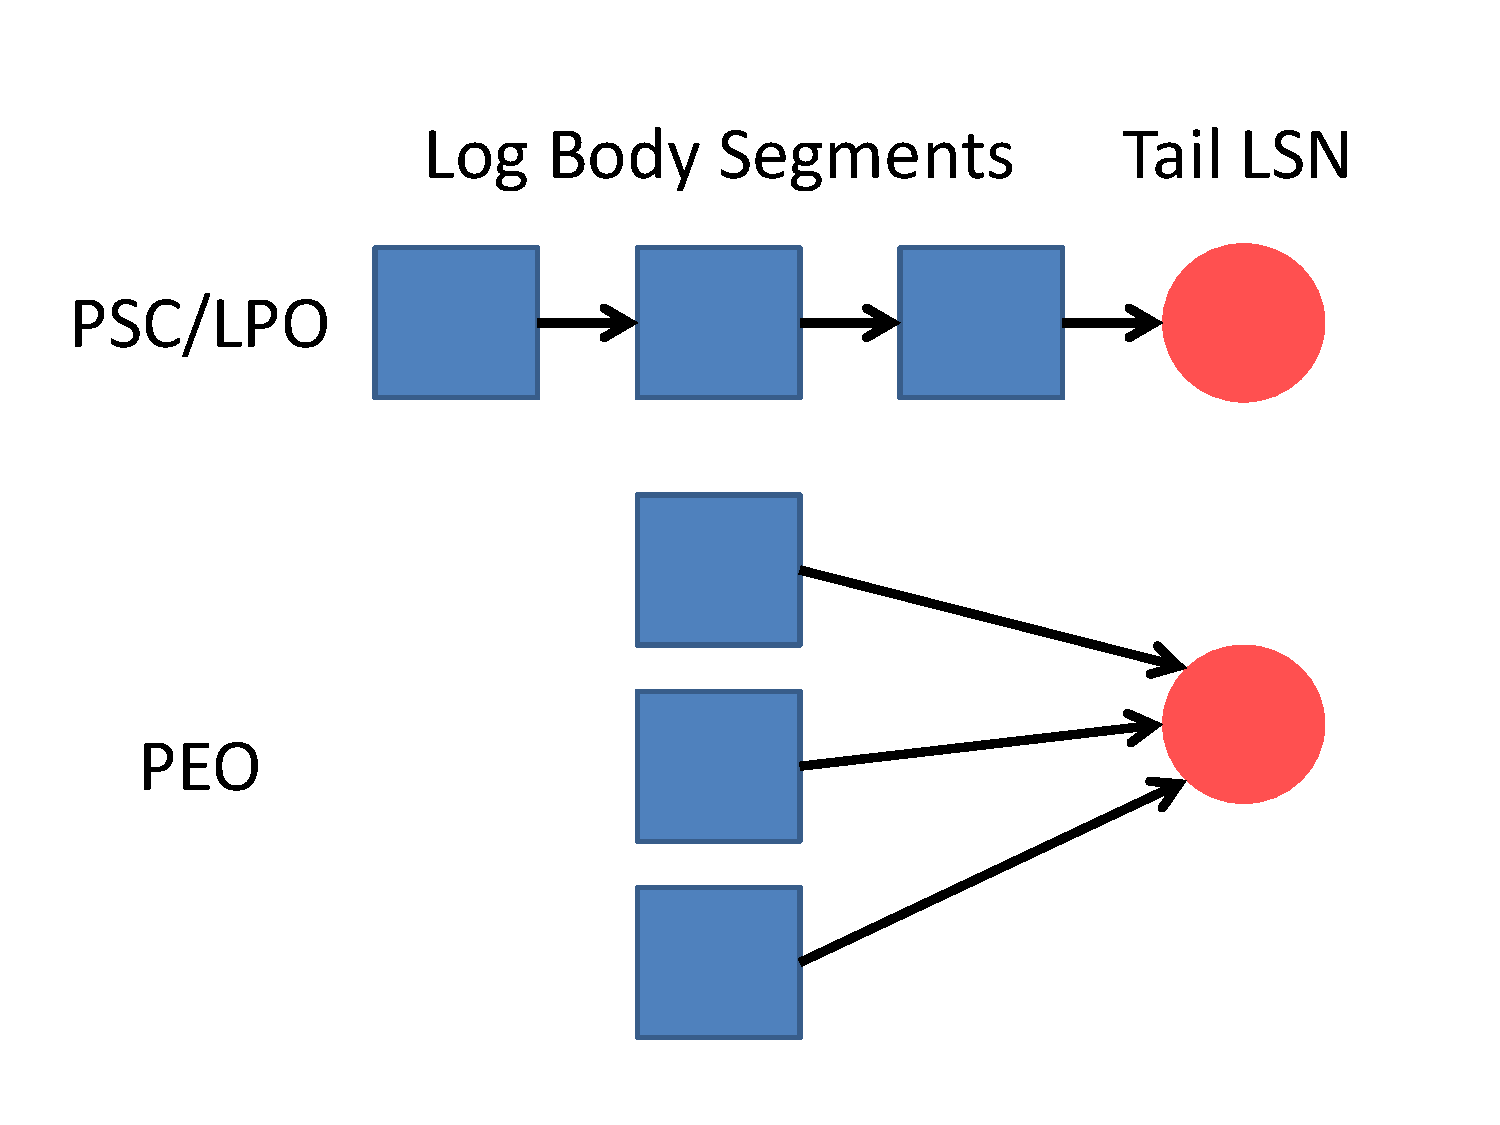
\includegraphics[width=.7\textwidth]{PMC/persist_wal.pdf}
\caption{\textbf{Partial Epoch Order.} PEO allows regions of NVRAM to persist in parallel while enforcing recovery correctness. \texttt{persist\_wal} persists entire log entry bodies in parallel using epochs.}
\label{fig:persist_wal_persist}
\end{figure}


TEO accelerates persists by decreasing persist critical path within threads, producing a sequential chain of dependencies, shown in Figure~\fixme{ref}.
With PSC/LPO all atomically persistable regions (usually 8 bytes) must persist in serial.
TEO relaxes this constraint, with the help of barriers, to persist log entry bodies in parallel, reducing persist critical path.
Cross-thread persist dependencies are relatively easy; no additional persist barrier is required.
This model is closest to existing work \fixme{cite BPFS}, which I discuss next.

\subsection{Byte Addressable Persistent File System}
\label{sec:PMC:PersistenceModels:BPFS}

The Byte Addressable Persistent File System (BPFS) \fixme{cite} is the de-facto standard for existing persistent memory consistency models, used additionally by \fixme{cite NVHeaps, IBM's logging, others?}.
Threads persist by writing to the persistent address space, enforcing persist order via epoch barriers.
BPFS additionally provides an example implementation, enforcing persist order with only cache modifications (little additionally buffering or modifications to the memory system).
A table of epochs is kept in the cache of each core, with each cache line keeping track of its persist epoch number.
The cache writes back in the background, making sure that each epoch persists completely before starting to write back the next epoch.

Data sharing and persist order is enforced strictly by stalling.
If at any point a thread overwrites a cache line from a previous persist epoch (even from the same thread), it stalls until the previous persist epoch completes persisting.
Further, if a thread reads a cache line from a previous persist epoch produced by a remote thread, it again stalls until the previous persist epoch completes persisting (it does not stall if the reading thread is the same as the producing thread).
Single threaded applications may persist data within epochs in parallel, and enforce correct cross-thread persist order (at the cost of stalls).

Aside from the performance implications of stalling, BPFS has several problems.
Specifically, there is no discussion of the memory consistency model, which produces \emph{correctness} problems.
I will demonstrate here that the implementation as described is susceptible to deadlock.

Consider Figure~\ref{fixme}.
Each thread runs a single epoch with two persists to shared memory.
The second thread executes these persists in opposite order of the first.
If thread 1 writes to A at the same time thread 2 writes to B a deadlock will occur.
Thread 1 attempts to write to B, fetching the cache line for B, realizing that thread 2 has not yet persisted, so thread 1's epoch must be ordered after thread 2's epoch.
Similarly, thread 2 attempts to write to A, ordering its epoch after thread 1's; a cycle has occurred, preventing forward progress.

This problem may occur even without data races or a total order on writes.
Imagine that A and B on each thread are different address, each protected by locks, but that thread 1's A (B) is on the same \emph{cache line} as thread 2's A (B).
Such \emph{false sharing} may produce performance problems for existing cache systems, but in the case of BPFS produces deadlock.
Furthermore, one might try to solve this problem by reordering thread 2's writes so that both thread 1 and thread 2 write in the same order, totally ordering the epochs (whoever accesses A first runs to completion while the other stalls).
However, relaxed consistency models may allow the processor (or compiler) to reorder writes and persists, arriving at the original problem.

I believe that the solution is to properly define the interaction between persistence and the consistency model.
BPFS gets into trouble because it assumes transaction-like persistence semantics without any rollback mechanism -- persistence and concurrency control are too tightly coupled without proper support.
My TEO is strongly influenced by BPFS but allows concurrent, conflicting epochs to make forward progress with either undefined behavior or behavior defined by the underlying consistency and persistent consistency models.

\section{Conclusion}
\label{sec:PMC:Conclusion}

This chapter motivated the need for more precise persistent consistency models to allow greater persist performance while providing an easy to program interface that enforces correct persist behavior.
I proposed three new persistent consistency models and relate them to existing work.
While this chapter has focused on persistence semantics and the programming interface, the next chapter demonstrates common persistent data structures, focusing on potential performance concerns.
